\chapter{Introduction}
\label{chapter1}

\section{Context}
Cloud computing has always been seen as a way of improving compute performance by the use of multiple computers connected to each other. The games industry has rapidly evolved along the years and a great deal of demand is apparent. Developers of games have pushed computer hardware to meet the needs of consumers for more complicated games and realism. Even with computer hardware becoming cheaper and more of a commodity, the costs of driving graphics rendering for high-end games to run at the optimal settings of 1080p at 60fps are still relatively high.

\section{Project Aim}
The aim of the project is to produce a solution which uses Software-Defined Networking to reduce the network latency in a network.

\section{Project Objectives}
\begin{itemize}
  \item A simple game program, that is computationally expensive enough to not perform optimally on a single machine (simple flight simulator with real time procedurally generated trees).
  \item A simplified cloud gaming system where the game created is launched on the cloud and input on the client side in the form of button presses on the keyboard is sent to the game on the server. The game frames produced are then sent to the client's screen.
  \item Produce a virtual network with simulated cloud game traffic and delay. With the use of SDN, reduce latency in the network.
\end{itemize}

\section{Deliverables}
The deliverables of the project include:
\begin{itemize}
  \item Code that demonstrates a simple game/simulation rendering graphics on a server and controlled by a client remotely.
  \item A manual on how to setup the client and server will be produced so the cloud gaming system can be easily setup and launched. 
  \item Code that will create a virtual network as well as a manual on how to set it up and run the code.
  \item Project report that explains the problem the project is trying to solve and the schematics of the solution produced as well as an evaluation of the solution.
\end{itemize}

\section{Project Schedule}
\begin{figure}[h]
 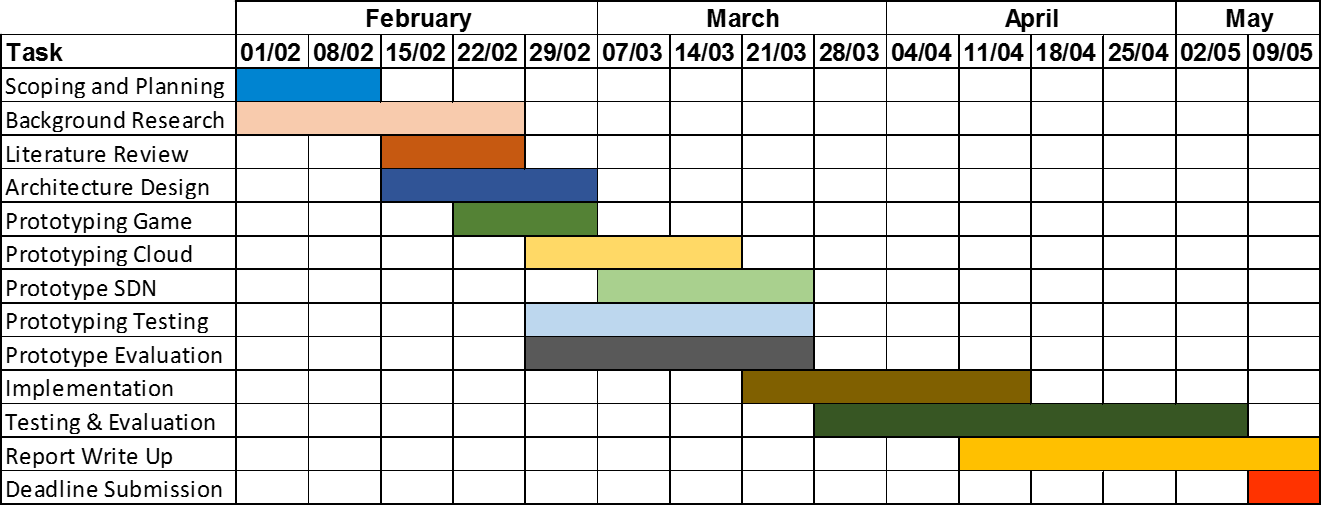
\includegraphics[width=\linewidth]{images/gantt.png}
 \caption{Gantt chart of project schedule}
 \label{fig:schedule}
\end{figure}

The approach that was used for this project was iterative. After doing background research, the next process is literature review of the information I have found. Comparisons of different techniques that will reduce latency and increase the overall performance of the system was made. A single technique was then chosen to focus on and this was software-defined networking. The next step was to design the architecture for the cloud gaming system along with how it will be implemented:
\newline
\par
A prototype of the game was produced and was made sure it was running properly on a single system in the DEC-10 Lab. The game rendered a procedurally generated tree using Lindenmayer system which is computationally expensive to produce in real time. The game also uses lighting and shadows which adds more to the compute power needed. The game area can be navigated around by the player using simple flight simulator controls.
\newline
\par
When this is completed, a server-client system where the server can receive user input from a client and relay the commands to the OpenGL program was prototyped. The intention of this was to stream the rendered frames in video format to the client's window and the bandwidth of the video traffic was to be recorded. Simulated traffic was then used on a virtual network for the SDN solution. Which was tested against different test scenarios and evaluated.